\documentclass[hidelinks,12pt]{article}
\linespread{1.3}
\usepackage{hyperref}
\usepackage{enumitem}
%\usepackage{enumerate}
\usepackage{changepage,lipsum,titlesec, longtable}
\usepackage{cite}
\usepackage{comment, xcolor}
\usepackage[pdftex]{graphicx}
  \graphicspath{{images/}, {images/stat/}}
  \DeclareGraphicsExtensions{.pdf,.jpeg,.png, .jpg}
\usepackage[cmex10]{amsmath}
\usepackage{tikz}
\usepackage{array} 
\usepackage{subfigure} 
\newcommand{\grey}[1]{\textcolor{black!30}{#1}}
\newcommand{\red}[1]{\textcolor{red!50}{#1}}
\newcommand{\fref}[1]{Figure \ref{#1}}
\newcommand{\tref}[1]{Table \ref{#1}}
\newcommand{\eref}[1]{Equation~\ref{#1}}
\newcommand{\cref}[1]{Chapter~\ref{#1}}
\newcommand{\sref}[1]{Section~\ref{#1}}
\newcommand{\aref}[1]{Appendix~\ref{#1}}

\renewcommand{\labelenumii}{\theenumii}
\renewcommand{\theenumii}{\theenumi.\\arabic{enumii}.}

\oddsidemargin0cm
\topmargin-2cm %I recommend adding these three lines to increase the
\textwidth16.5cm %amount of usable space on the page (and save trees)
\textheight23.5cm

\makeatletter
\renewcommand\paragraph{\@startsection{paragraph}{4}{\z@}%
            {-2.5ex\@plus -1ex \@minus -.25ex}%
            {1.25ex \@plus .25ex}%
            {\normalfont\normalsize\bfseries}}
\makeatother
\setcounter{secnumdepth}{4} % how many sectioning levels to assign numbers to
\setcounter{tocdepth}{4}    % how many sectioning levels to show in ToC


\begin{document}
\title{SEED project\\
       \large Reading Documentation and Getting Started}
\maketitle
\tableofcontents
\newpage
\section{Intro}\label{sec:intro}
Developed based on DOE SEED (Standard Energy Efficiency)
platform~\cite{DOESeed2015}. The platform is open source. The data is
confirmed to Building Energy Data Exchange Specification (BEDES)
taxonomy. 
\begin{itemize}
\item real-time
\item robust (testing)
\end{itemize}

Input: 

\begin{itemize}
\item sub-meter data ``Utility submetering is the implementation of a
system that allows a landlord, property management firm, condominium
association, homeowners association, or other multi-tenant property to
bill tenants for individual measured utility usage''(wikipedia)

\item Green Button: 15min time step energy data 

  \begin{itemize}
  \item ``Green Button data implements the North American Energy
    Standards Board's \textbf{(NAESB) REQ 21 -- Energy Service Provider
    Interface (ESPI) energy usage information exchange standard}.''
    ~\cite{GreenButton2015}

  \item General: ``The presence of a Green Button certification mark
    on an energy provider's website enables consumers and application
    developers to confidently rely on the data they receive being
    Green Button standard compliant.''
  
  \item ``Green Button \textbf{Download My Data} provides downloadable
    energy data that complies with the Green Button standard ensuring
    a consistent data format from all energy provider websites.''
  
  \item ``Green Button \textbf{Connect My Data} provides application
    developers an automated technique to access consumer energy
    information while providing consumers security.''
  \item target: 15min Green Button CMD, commercial building

  \end{itemize}
\end{itemize}

RESTful API ensure compatibility with the existing PostgreSQL
\section{Procedure}
Our goal: add in Green Button energy data (15-min time-step) to SEED

\begin{figure}[h!]
  \centering
  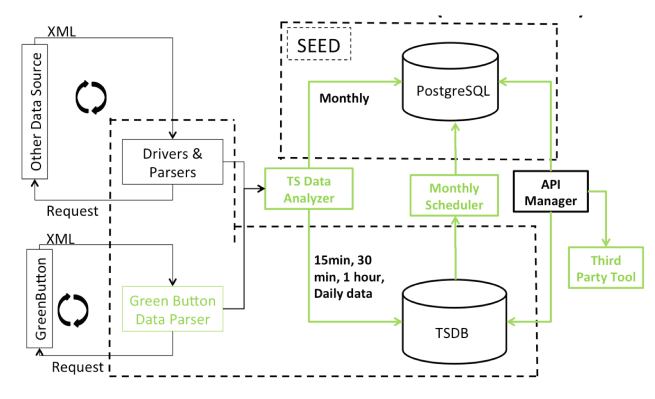
\includegraphics[width=0.7\linewidth]{diagram.png}
  \caption{Diagram of the SEED project~\cite{SEEDProjectPlan}}
  \label{fig:diagram}
\end{figure}

Components:
\begin{verbatim}
- Driver: request energy usage data in XML format (through DMD or CMD)
- Parser: XML (NAESB-ESPI) --> SEED time series (BEDES standard)
  *   import
  *   convert
      - mapping: raw data to columns in SEED
      - matching: data to building, using BuildingSnapshot_id <-> meter_id
- PostgreSQL Database (existing): receive SEED time series
  *   a table for each building
  *   group info tables (??)
  *   two groups of table: 
        time: monthly data of a year
        building: monthly data of a building
- TSDB
  *   {timestamp, reading, tags = {unit, type, meter_id, ...}}
      note: timestamp example: 2005-10-30 T 10:45 UTC
  *   "A time series database (TSDB) is a software system that is
optimized for handling time series data, arrays of numbers indexed by
time (a datetime or a datetime range)."(wikipedia)
  *   In the current case, time series are labeled with tags  
  *   why using it? relation table has the following problems:
        difficult to create group info table (P13)
        difficult for inter-table query
        data storage design coupled with queries
  *   OpenTSDB and InfluxDB
- TS (Time Series) Data Analyzer (redirecting BEDES data): 
 detect time interval
  *   receive data (BEDES standard) from "Green Button Data Parser" and
  other sources with data in BEDES standard
  *   detect utility type
  *   get information from PostgreSQL (out of Green Button Parser??)
  *   insert data with time stamp and information from PostgreSQL into TSDB
  *   filtering data and quality check (??)
  *   send monthly data to PostgreSQL send others to TSDB
- Monthly Scheduler: aggregate data in TSDB to Monthly and push it to PostgreSQL
  *   query TSDB
  *   aggregate TSDB data to monthly
  *   push the (aggregated data, meter_id) to the right BuildingSnapshot in SEED PostgreSQL
- API Management Platform: connect with different services, APIs and third-party apps

possible components: 
- Adapters that transfer SEED request to TSDB request and parse TSDB
return value to SEED
 
\end{verbatim}

\section{Function Specs}
\begin{verbatim}
# property list -> building_id list
# requires: for all x in property_list, x valid property ??
         or exists x in property_list, x valid property ??
# ensures: for all y in building_id list, for all x in property_list
           y.x is True
or 
# ensures: for all y in building_id list, for all VALID x in 
           property_list, y.x is True
get_buildingsnapshot_id(property_list);

## ## ## ## meter_building_snapshot table (where ??) ## ## ## ## ##
# (buildingsnapshot_id, time_start, time_end, time_interval) -> 
  (timestamp, reading, energy_unit) list
# requires : buildingsnapshot_id valid ??
             time_start <= time_end,
             time_interval in {15min, 30min, day, month}
             
# ensures: for all [t, r, e] in \result, time_start <= t < time_end
(?? inclusive or exclusive)
(?? do not differ different energy utility type?)
# assume if time start and end are out of boundary, return the whole
table.

get_building_monthly_energy_data(buildingsnapshot_id, time_start,
time_end, time_interval)

get_buildings_monthly_energy_data(buildingsnapshot_id_list ,
time_start, time_end, time_interval);

## ## ## ## ## ## ## ## TSDB ## ## ## ## ## ## ## ## ##
(?? what is property_list here ?? buildingsnapshot_id ??) (P20)
# get_building_finer_monthly_energy_data(property_list, time_start,
time_end, time_interval);

# get_building_finer_monthly_energy_data(buildingsnapshot_id ,
time_start, time_end, time_interval);

# get_buildings_finer_monthly_energy_data(filter_list , time_start,
time_end, time_interval);

## ## ## ## ## ## ## ## TSDB and m_b_s table ## ## ## ## ## ## ## ## ##
# get_buildings_finer_monthly_energy_data(buildingsnapshot_id_list ,
time_start, time_end, time_interval);

## ## ## ## ## ## ## ## other ## ## ## ## ## ## ## ## ##
# filter_list -> snapshot_id list
get_buildingsnapshot_ids(filter_list)

Data structure:

## Building filter data structure ##
(?? what is it used for ? what operations it can have ?)
if is_range: 
    property_value_list = [range_start, range_end]
else:
    property_value_list = anything
    
typedef [property_name, property_value_list, is_range] filter
\end{verbatim}

\section{Question}
\begin{enumerate}
\item Why little modification to the SEED platform will encounter
  scalability issue? (P6)
  
\item The performance difference of relational and time-series
  database (http://www.javaworld.com/article/2078664/java-app-dev/10-things-never-to-do-with-a-relational-database-.html)(P11)
  
\item RESTful API?
\item ``get information from PostgreSQL '' (P11)
  is the meter\_id information in the output of Green Button Parser?
  
No, the meter\_id is got from SEED.BuildingSnapshot (P12)
  
\item What's the ``quality checks''?
\item what's group info tables in PostgreSQL?
\item Code specs: 

probably need more clear specs ? especially for cases involving potential exceptions?

type specifications of the functions might be needed.
\item The data mapped in GIS

\end{enumerate}

\section{Definitions}
\begin{itemize}
\item Smart meter: sample energy usage at 15min interval (half), other
  intervals include 30min, one hourly, daily, monthly
\item XML: Extensible Markup Language. XML has come into common use
  for the interchange of data over the Internet. For example, Scalable
  Vector Graphics (SVG) in graphics is is an XML-based vector image
  format for interactivity and animation. (Wikipedia)
\item PostgreSQL: a object-relational database management system
  (ORDBMS), which is an object-oriented version of relational
  database. A relational database organize the data based on the
  relational model, which is consistent with first-order logic. In the
  relational model, data is represented as tuples. If each row
  represents a data entry and each column represents an attribute of
  the data entry, then each row is a tuple in the relation R defined
  by the database.

  Side: from the lecture notes of 15-251, an axiomatic system consists
  of axioms, deduction rules and theorems (detuctible from axioms
  using deduction rules). 0th order logic is the logic consisting of
  propositions (propositional variable) and symbols as
  $(, ), \neg, \land, \lor, \implies, \iff$. The first-order logic is
  0th order logic together with quantifiers.

\item RESTful: ``Web service APIs that adhere to the REST architectural
  constraints are called RESTful APIs''(wikipedia)
\item relational database management system (RDBMS)
\item REST
  \begin{itemize}
  \item web service: ``A web service is a collection of open protocols
    and standards used for exchanging data between applications or
    systems.''~\cite{REST2015}
  \item ``Web services based on REST Architecture are known as RESTful
    web services.''~\cite{REST2015}
  \item REST architecture: 
    \begin{itemize}
    \item server: provide resources
    \item client: access and present resources
    \end{itemize}
  \end{itemize}
\item REST: REpresentational State Transfer, it uses HTTP method (GET,
  PUT, POST etc) for data communication.
\item TSDB: ``TSDBs are databases that are optimized for time series
  data. Software with complex logic or business rules and high
  transaction volume for time series data may not be practical with
  traditional relational database management systems.'' (wikipedia) so
  in our case, it has ``high transaction volume''
  
\item EPA Energy Star categorization(lookup !!)
\end{itemize}

\newpage
\bibliographystyle{plain}
\bibliography{myCitation}
\end{document}